\documentclass{article}
\usepackage[utf8]{inputenc}
\usepackage{booktabs}
\usepackage{longtable}
\usepackage{graphicx}
\usepackage{float}

\begin{document}

\title{MAS Task 1}
\author{Denis Uzhva}
\date{October 2019}
\maketitle

\begin{figure}[H]
    \centering
    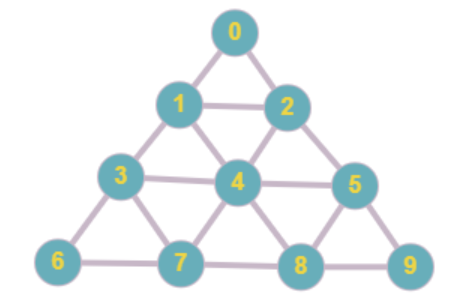
\includegraphics[width=.6\textwidth]{triangleTen.png}
    \caption{Topology of the graph}
    \label{fig:gr}
\end{figure}

Root node: 0. Cost of a memory cell: 10\$, cost of a message: 0.01\$, cost of a Data Center call: 1000\$.

\begin{scriptsize}
\begin{longtable}{lllllllllll}
	\toprule
	N	&	M	&	K	&	T	&	Mem.	&	Comp.	&	Sum.		&	Mul/Div	&	Local Cost	&	DC Cost	&	Total Cost	\\
	\midrule
	10	&	36	&	3	&	56	&	2*10+3	&	2		&	2*(10-1)	&	1		&	230.56		&	1000	&	1230.56		\\
    \bottomrule
	\caption{N -- num. of nodes, M -- num. of connections, K -- depth, T -- time (num. of messages sent), \
		Mem. -- memory (1 array with nodes, 1 array with roots, 3 variables with agent IDs: self, root and previous), \
		Comp. -- num. of comparisons, Sum. -- num. of sums, Mul/Div -- num. of multiplications and divisions, \
		Local cost -- cost of everything within the graph, DC Cost -- cost of all the calls to our Data Center, \
		Total Cost = Local Cost + DC Cost}
	\label{tab:acc}
\end{longtable}
\end{scriptsize}

\end{document}
